\documentclass{article}

\usepackage[hangul]{kotex}
\usepackage{amsmath}
\usepackage{tikz}
\usepackage{minted}
\usepackage{geometry}
\usepackage{enumitem}
\usepackage{multicol}
\usepackage[linguistics]{forest}
\usepackage{algorithm}
\usepackage{algpseudocode}
\usepackage{hyperref}

\hypersetup{
  colorlinks   = false, %Colours links instead of ugly boxes
  urlcolor     = blue, %Colour for external hyperlinks
  linkcolor    = black, %Colour of internal links
  citecolor   = red %Colour of citations
}

\geometry{
  a4paper,
}

\setmonohangulfont{D2Coding}

\title{프로그래밍과 문제해결 \\ Assignment \#1}
\author{무은재학부 박재원 (2024****)}
\date{\today}

\begin{document}

\begin{titlepage}
	\centering
	{\huge CSED101 프로그래밍과 문제해결\par}
	\vspace{0.5cm}
	{\LARGE Assignment \#1\par}
	\vspace{0.5cm}
	{\large \today\par}
	\vfill
  
  \begin{multicols}{2}
    \vphantom{}
    \columnbreak
  {
    \Large 
    \begin{description}[nosep, align=right, labelwidth=\widthof{00000000000000000}]
      \item[학과] 무은재학부
      \item[학번] 2024****
      \item[이름] 박재원
      \item[POVIS ID] ****
    \end{description}
  }
  \end{multicols}

  \vspace{1cm}


  \begin{quote}
    명예서약 (Honor code)

    ``나는 이 프로그래밍 과제를 다른 사람의 부적절한 도움 없이 완수하였습니다.''
  \end{quote}

\end{titlepage}

\tableofcontents

\section{개요}

본 과제는 Wordle 게임을 파이썬으로 구현하는 것이다.
Wordle 게임은 임의로 정해진 5글자 길이의 영단어를 맞추는 게임이다.
사용자는 총 6번의 시도 안에 정답을 맞추어야 한다.
각 시도에 입력하는 단어는 5글자 길이의 유효한 단어여야 하며,
입력한 단어가 오답일 경우, 각 알파벳의 배경색을 3가지 색 중 한가지로 칠함으로써 힌트를 제공한다.

\section{설계}

\subsection{구조도}

프로그램의 전체 구조도는 그림 \ref{fig:structurechart}와 같다.

\begin{description}
  \item[입력부] 사용자 추측 단어 입력, 게임 계속 진행 여부 입력, 단어 리스트 파일 읽기
  \item[처리부] 입력 단어 유효 여부 판단, 정답 여부 판단, 힌트 결정 등
  \item[출력부] 현황판, 안내 메시지, 오류 메시지 출력 등
\end{description}

\begin{figure}
  \centering
  \begin{forest}
    for tree={
      draw,
      grow=east
    }
    [main
      [load\_word\_list]
      [run\_game
        [input\_word
          [is\_valid]
        ]
        [print\_status
          [get\_colored\_string
            [get\_colored\_char]
          ]
        ]
        [is\_correct]
      ]
    ]
  \end{forest}
  \caption{본 프로그램의 전체 구조도}
  \label{fig:structurechart}
\end{figure}

\subsection{알고리즘}
프로그램의 알고리즘을 의사코드로 나타내면 알고리즘 \ref{alg:all}\과 같다.

\begin{algorithm}
  \caption{본 프로그램 주요 부분의 의사 코드} \label{alg:all}
  \begin{algorithmic}
    \State 정답단어 $\gets$ 단어 리스트에서 랜덤으로 선택한 단어
    \While {}
      \Repeat
        \State 단어 입력받기
        \State 입력 단어를 모두 소문자로 바꾸기
        \If {입력단어 $=$ quit}
          \State 게임 한 판 종료하기.
        \ElsIf {입력한 단어가 유효하지 않은가}
          \State 에러 메시지 출력
        \EndIf
      \Until 유효한 단어인가

      \If {입력단어 $=$ 정답단어}
        \Comment {게임 성공}
        \State 정답 공개 \& 게임 한 판 종료.
      \Else
        \State history에 입력단어 추가 \& life 감소
        \If {life $\leq 0$}
          \Comment 게임 실패
          \State 정답 공개 \& 게임 한 판 종료.
        \EndIf
        \ForAll {$word \in history$}
          \Comment 현황판 출력
          \ForAll {$char \in word$}
            \If {char가 정답단어의 같은 위치에 있는가}
              \State 초록색 배경과 대문자로 글자 출력
            \ElsIf {char가 정답단어에 포함되어 있는가}
              \State 노란색 배경과 대문자로 글자 출력
            \Else
              \State 회색 배경과 대문자로 글자 출력
            \EndIf
          \EndFor
          \State 줄바꿈 출력
        \EndFor
        \State 남은 시도 횟수만큼 빈 칸 출력
      \EndIf
    \EndWhile
  \end{algorithmic}
\end{algorithm}

\section{실행 방법 및 예제}

본 과제는 MacOS\footnote{특정 OS에 종속적인 기능을 사용하지 않으므로 다른 운영체제에서도 정상 작동하리라 예상된다.}, CPython 3.12.2에서 작성 및 테스트되었다.

본 과제를 실행하려면 우선 다음과 같이 assn1.py와 word\_list.txt를 같은 디렉토리에 위치시킨 후,
파이썬 코드를 실행시키면 된다. 이후 출력되는 메시지에 따라서 적절히 입력값을 입력하면 된다.
\begin{minted}[]{bash}
  ls
  # assn1.py      word_list.txt
  python assn1.py
  # Wordle game starts!
  # ...
\end{minted}

실제 프로그램 실행 모습은 아래와 같다.

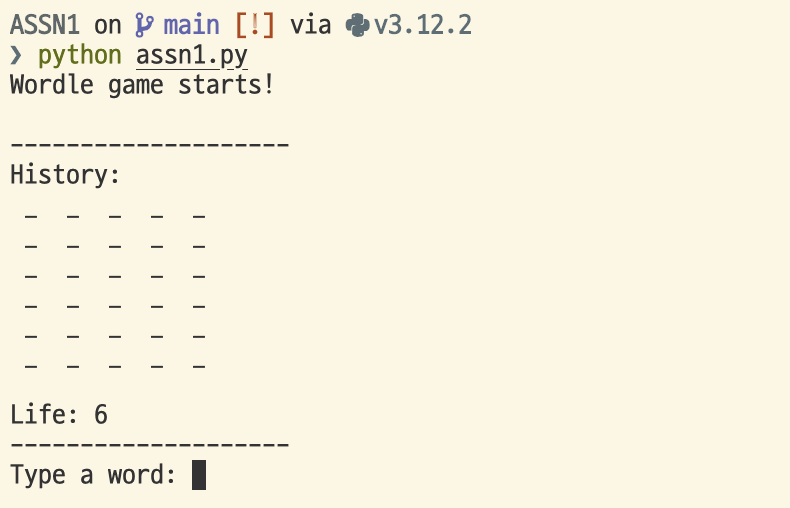
\includegraphics[width=5cm]{start.png}

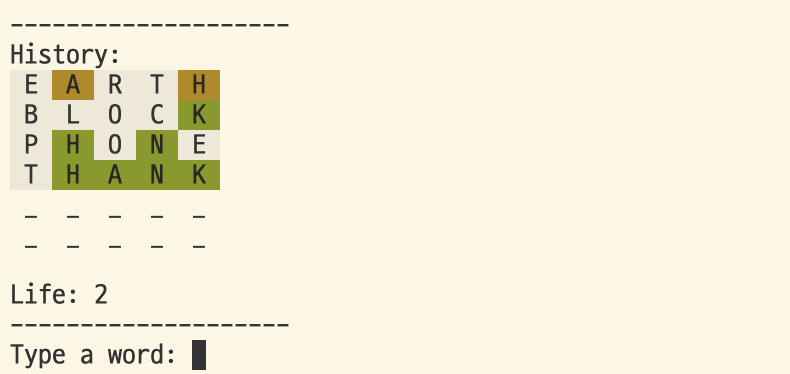
\includegraphics[width=5cm]{middle.png}

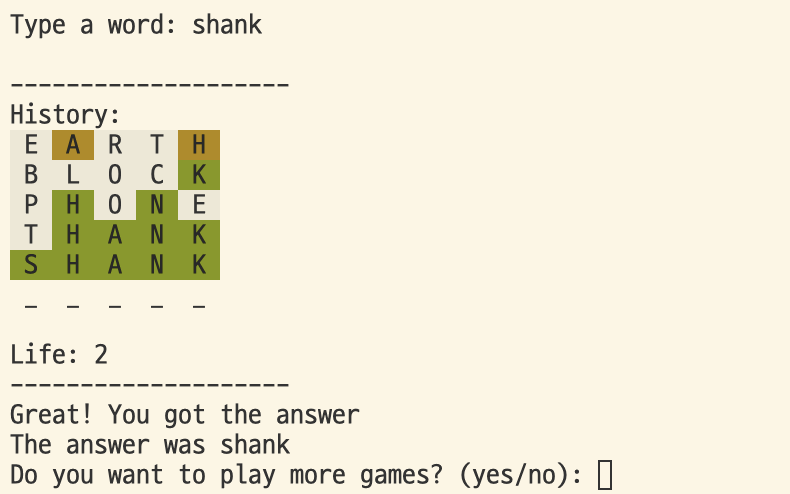
\includegraphics[width=5cm]{end.png}

위 스크린샷은 정답 단어가 shank일 경우이다.
각 입력 단어에 대해서 적절한 힌트를 제공하고, 정답을 맞출 경우 정답이라는 메시지를 출력하며
게임이 종료된다. 이후 다시 플레이 할지 여부를 물어본다.

\section{토론}

\subsection{is\_valid 함수}
문서에 따르면 유효하지 않은 입력일 경우, 각 종류에 따라 다른 오류 메시지를 출력해야 했다.
이는 입력의 유효성을 판단하는 is\_valid 함수와 분리될 수 없지만,
is\_valid 함수 안에서 출력을 하는 것은 함수의 목적에 맞지 않는다고 판단했다.
따라서 문서에서 제안된 정의처럼 단순히 bool 값만 반환하는 것이 아니라 오류 메시지도 함께 튜플로 반환하도록
구현하였다. 
\begin{minted}[]{python3}
return (False, "Input word is not a five-letter word!")
\end{minted}
와 같이 (bool, string) 형태로 반환한다.

\subsection{input\_word 함수}
사용자로부터 추측 단어를 입력받는 로직이 단순하지 않기
때문에 별도 함수로 분리했다.

또한 입력이 유효하지 않을 경우 계속 다시 입력을 받아야한다.
이를 구현하기 위해서 우선 반복문(while True) 내에서 계속해서 입력을 받고,
입력이 유효한 경우, break문으로 반복문을 탈출하도록 구현했다.

\section{결론}

본 과제를 통해 조건문과 반복문을 다양한 상황에서 여러 로직을
구현하기 위해 사용해보며 제어문에 더욱 익숙해 질 수 있었다.
또한 사용자 정의 함수를 통해 코드를 더욱 효율적으로 작성하는 방법을
익힐 수 있었다. 랜덤 모듈을 통해 랜덤한 값을 사용하고 테스트하는 방법도
익혔다.

\section{개선 방향}

현황판을 출력할 때, 매 번 조건문을 통해 어떤 배경색을 칠할지 정하고 있다.
하지만 이전에 입력했던 단어의 경우 칠해야 하는 배경색도 매 번 같으므로,
그 때 그 때 다시 판단하는 것은 비효율적이다. 따라서 처음 단어가 입력되었을 때
한 번만 칠해야 할 색을 정해서 다른 변수에 저장해 두었다가,
현황판을 출력할 때는 그 저장된 값을 출력만 하도록 개선하면 더욱 효율적으로
구현할 수 있으리라 예상된다.

\end{document}  